\documentclass{article}


\usepackage{arxiv}

\usepackage[utf8]{inputenc} % allow utf-8 input
\usepackage[T1]{fontenc}    % use 8-bit T1 fonts
\usepackage{hyperref}       % hyperlinks
\usepackage{url}            % simple URL typesetting
\usepackage{booktabs}       % professional-quality tables
\usepackage{amsfonts}       % blackboard math symbols
\usepackage{nicefrac}       % compact symbols for 1/2, etc.
\usepackage{microtype}      % microtypography
\usepackage{lipsum}
\usepackage{multirow}
\usepackage{graphicx}


\title{Artist Identification	\\  A comparison between AlexNet, GoogLeNet and ResNeXt}


\author{
  Mattia Bottaro \\
  Dipartimento  di Matematica\\
  Università di Padova \\
  \texttt{mattia.bottaro@studenti.unipd.it} \\
  %% examples of more authors
   \And
  Mauro Carlin \\
Dipartimento  di Matematica\\
Università di Padova \\
\texttt{mauro.carlin@studenti.unipd.it} \\
  %% \AND
  %% Coauthor \\
  %% Affiliation \\
  %% Address \\
  %% \texttt{email} \\
  %% \And
  %% Coauthor \\
  %% Affiliation \\
  %% Address \\
  %% \texttt{email} \\
  %% \And
  %% Coauthor \\
  %% Affiliation \\
  %% Address \\
  %% \texttt{email} \\
}

\begin{document}
\maketitle

\begin{abstract}
	\textit{In this essay we present our work for the project of the Cognitive Services course.
	The problem we face is the artist identification, that is being able to recognize the author of a painting, given an image of it. Our dataset consists of about 10.000 paintings of 23 different artists.
	In order to resolve this task, we have exploited some famous Convolutional Neural Networks (CNNs), i.e. AlexNet, GoogLeNet and ResNeXt, that come with \textit{Pytorch} library. Those networks have been trained according to two distinct approaches: training them from scratch or exploiting pre-trained models using transfer learning technique. We used \textit{Google Cloud Platform} to train and evaluate our models.\\
	What we have achieved is a set of results which are in line with the state-of-the-art, confirming that CNNs are suitable to solve this type of task.}
\end{abstract}


% keywords can be removed
\keywords{Convolutional Neural Networks \and Artist Identification \and CNNs \and ResNeXt \and GoogLeNet \and AlexNet \and Transfer Learning}


\section{Introduction}
Artist identification is a task regarding recognition of the painter who depicted a certain painting, given an image of it.\\
It's still nowadays a difficult problem to solve, for the following reasons:
\begin{itemize}
	\item there are not many contributions yet and these rely on the latest models of deep learning (e.g. CNNs);  \textbf{SISTEMARE, USANO APPROCCI VECCHI}
	\item the available datasets are not as large as those used by models which solve more common tasks, such as image classification;
	\item an artist's style can change a lot through his works, or it could be influenced by other painters. \textbf{QUESTO RENDE LA CLASSIFICAZIONE UN TASK PARTICOLARMENTE COMPLICATO}
\end{itemize}
This type of task is still done by art experts and contributions to this type of problem can help and lead to the development of automatic fake artifact detection and automatic cataloguing of artworks.\\
We used three different CNNs: AlexNet (2012), GoogLeNet (2014) and ResNeXt (2016). For each of them, we have established two different ways of training: from scratch and with transfer learning  upon pre-trained version of such CNNs. Then we have observed and compared their performance. From our experiment we have obtained 83.768\% accuracy.\\


The rest of the essay is structured as follows: In section \ref{relwor} we discuss  similarities and differences between previous works and ours. In section \ref{dataset} we explain which dataset we have used, how it was formed and which preprocessing and data augmentation techniques we have exploited. In section\ref{method} we exhibit the CNNs' architectures and how we have trained them. In section \ref{experiments} we show some details regarding the \textit{GCloud Compute Engine}'s configuration, the metrics used to assess the goodness of the models and the detailed results of this experiment. Finally, in section \ref{conclusions} we draw some conclusion and we outline some possibile future works which rely on our result.


\section{Related Works}\label{relwor}

In this section we show some previous works related to ours. In addition to defining the references our experiment, the following should further convince the reader of present-day difficulty in achieving good precision in artist identification.\\
Recently CNNs have become widespread, this is due to the good performance and results obtained in this kind of task. In fact, we can distinguish the contributions to this task between those that come before the spreading of the CNNs, and thus do not use them, and those that instead benefit from it.\\
In our problem, the features that characterize an artist's style can be many and difficult to engineer, such as texture, shape, color, tone, variety, proportion, pattern and brush strokes.\\
Instead, it is well known that CNNs are able to learn those features that characterize an image, without having to identify and engineer a set of characterizing features.\\
In works prior to CNNs, some famous approaches of detection features are exploited, such as Scale Invariant Feature Transforms (SIFT) and Histograms of oriented gradients (HOG) (\cite{Saleh2015}, \cite{mensink2014}, \cite{lombardi05}, \cite{jou2011}). These works have in common the use of an SVM 1-vs-rest classifier, except \cite{jou2011} which uses both SVM 1-vs-rest and Naïve Bayes classifier.\\ However, \cite{lombardi05} and \cite{jou2011} face the problem of style recognition, which is different than artist identification.\\
In addition, some of these perform on small or not so heterogenous datasets, such as \cite{mensink2014} which uses the artwork of a single museum, or \cite{jou2011} which focuses on only 5 artists. Instead, in our work we focus on recognizing 23 different artists, and for each of them we take the same number of artifacts (\cite{ArtGANDataset}). \\

One of the results achieved in \cite{hong2017} shows the actual improvement of performance in the use of CNNs up to 13.6\% more than SIFT, HOG or similar.  This work aims to detect artwork that violates copyright terms in television programs, TV series, movies or similar scenarios. They use different techniques to distort the images on their dataset, which would not be suitable for our context. They experiment with three different CNNs inspired by AlexNet and VGG, then they trained them from scratch with a weights' initialization according to a Gaussian distribution. In our work, instead, we use pre-existing CNNs. \cite{hong2017} is one of the few works which does not use SVM as classifier, but 3 Fully Connected Layers, and the last of them is a Soft-Max layer.\\
Other works like \cite{Bar2014} and \cite{razavian2014} use a CNN to generate features, then use an SVM 1-vs-rest classifier on top of it.
\cite{ArtistIdCNN406} exploit one of the most recent CNNs: ResNet-18 (\cite{resnet}). It is an ancestor of ResNeXt (\cite{resneXt}), one of the CNNs used in our experiment. As in our work, also in \cite{ArtistIdCNN406} either training from scratch and training through transfer learning are studied.
\\

In the latest years, the number of CNNs for visual recognition task is growing, as well as their contributions in the field of computer vision. What is missing is a performance comparison between the latter models in the field of artist identification and, more generally, in art-recognition tasks. This comparison is the purpose of our work.


\section{Dataset}\label{dataset}
\subsection{Overview}\mbox{}\\
The first requirement to train a CNN for artist identification is a dataset, of paintings of different artist, as large as possible. For our project we obtain a dataset from \cite{ArtGANDataset}, which is a subset of the WikiArt Dataset. \\
The dataset contain about 19,000 images of 23 different artists, regarding very different styles, genres  and epochs. There are also three .csv files that labeled all the paintings for genre, style, and artist: for our work we have used only the last one.\\ \\
In order to obtain a balanced dataset, we decided to select randomly 450 paintings for each artist, so in the end our dataset consists of 10,350 total images. \\
The next step was to divied the entire dataset in training, validation and test set. \cite{ArtGANDataset} suggests a possibile partition, but we decided to create our own because there isn't a test set in their repository, and some paintings included in the training set are also in the validation set, 
fact that can create a distorted evaluation of our model during training. Therefore, we split the dataset in training, validation and test sets using a 80-10-10 division per artist, obtaining a training set of 360 paintings per artist, and a validation and test sets each of 45 paintings per artist.

\subsection{Preprocessing and Data augmentation}\mbox{}\\
CNNs require a precise size for the images passed in it, so we had to modify the paintings in the dataset, considering that they vary widely in shape and size.\\
So, first, we take a 224$\times$224 crop of each input images, next we zero-center and normalize them, with mean and standard deviation calculated for each of the three channels red, green and blue (they are RGB images).  \\
During training we also randomly horizontally flip the image with a probability of 50\%, and also take a random crop of it (not always the central pixels), for essentialy two reasons:
\begin{itemize}
	\item randomness create variety and can avoid overfit;
	\item we assumed that the style of an artist is present everywhere in the painting, so taking random crops do not influence the performance of our models.
\end{itemize}
Instead, for validation and test sets we always have taken a central crop, in order to obtain stable results not depending on crop position.

\section{Method}\label{method}
In our work we have considered three different CNNs: AlexNet, GoogLeNet and ResNeXt. Every network we use takes as input a
3$\times$224$\times$224 RGB image and outputs the scores for each of the 23 artists present in our dataset.
\\
For all of our networks, we use a softmax classifier with
cross-entropy loss:
\begin{equation}
L_{i}=-\log \left(\frac{e^{f_{y_{i}}}}{\sum_{j} e^{f_{j}}}\right)
\end{equation}
\textbf{SPIEGARE}

First, we have trained the networks from scratch, in order to allow the network to learn features solely for our specific task of artist identification. \\
Afterwards, starting from networks with weights pre-trained on ImageNet dataset, we trained them using transfer learning to understand if a feature representation from ImageNet is a valuable starting point for our problem.\\
In both approches, we replaced the last fully-connected layer of the CNNs with a new one to calculate a score for each artist in
our dataset. We used \cite{pytorchguide} as a guide for replacing the fully-connected layer, and for performing transfer learning on the pre-trained networks.

\subsection{AlexNet}
AlexNet was the winning entry in ILSVRC 2012. It solves the problem of image classification where the input is an image of one of 1000 different classes (e.g. cats, dogs etc.) and the output is a vector of 1000 numbers, achieving a top-5 error of 15,8\%.
Architecture (Figure \ref{fig:alexnet}) is made up of eight layers, five convolutional, some of them followed by max pooling layers, and three fully-connected, with ReLU as activation function.\\
AlexNet also uses dropout, introduced in 2012 in \cite{dropout}, to reduce overfitting. In dropout, a neuron is dropped from the network with a probability of 0.5. When a neuron is dropped, it does not contribute to either forward or backward propagation. 
As a result, the learnt weight parameters are more robust and do not get overfitted easily.\\
We decided to include AlexNet in our work because it represent the starting point of image classification with CNN, so it would be iteresting to compare its performance on our task with more recent, complex and deep networks.

\begin{figure}[h]
	\centering
	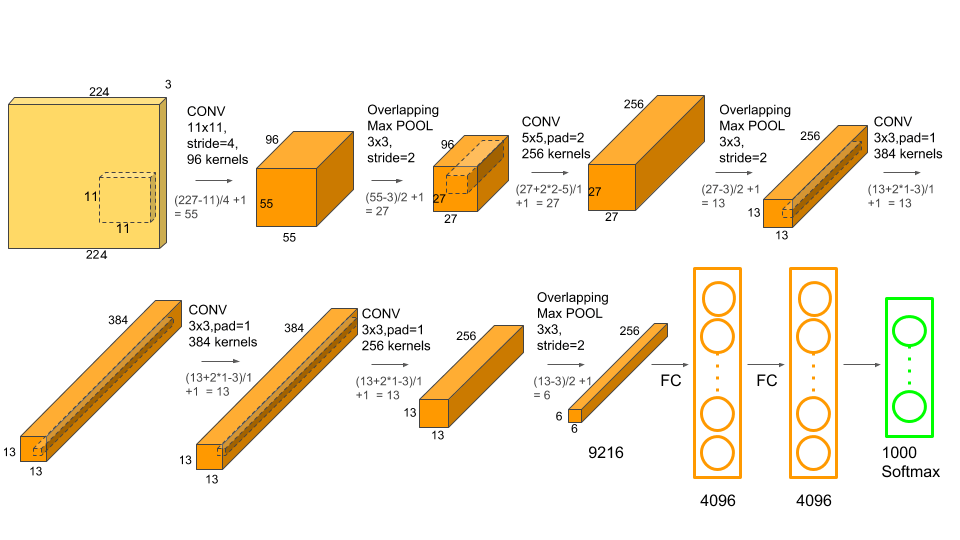
\includegraphics[width=0.7\linewidth]{image/AlexNet}
	\caption{AlexNet's architecture}
	\label{fig:alexnet}
\end{figure}

\subsection{GoogLeNet}
GoogLeNet won the ILSVRC 2014 achieving 6.67\% top-5 error on ImageNet. We considered this netowrk in our work PERCHè HA OTTENUTO IMPROVMENT NOTEVOLE DALL'ANNO PRECEDENTE, QUINDI INTRODUCENDO INNOVAZIONE CHE EFFETTI AMENTE FUNZONAO.
It is composed of 22 layers, with different innovations regarding the fully-connected layers, the vanishing gradient problem and a new inception module.\\
An interesting addition to the architecture is to change the second last fully-connected layer with an average pooling layer. This layer spatially averages the feature map, converting 7x7x1024 input to 1x1x1024, reducing the computation and the number of parameters, by a factor of 49. This average pooling layer is finally followed by a normal fully-connected layer with 1000 neurons (and 1024x1000 parameters), for the 1000 ImageNet classes.
During training, to address the vanishing gradient problem, special extra structures are added to the network (these are removed during testing). These are auxiliary classifiers attached to intermediate layers. All the losses from each classifier gets added up, taking contribution from the auxiliary classifier lower
than the main one, during training. The gradient from the main classifier which would have otherwise become very small, and thus slowing training, by time it reached the lower initial layers, receives gradient from the auxiliary classifiers and thus the net gradient becomes big enough to allow training to progress.
\begin{figure}[h]
	\centering
	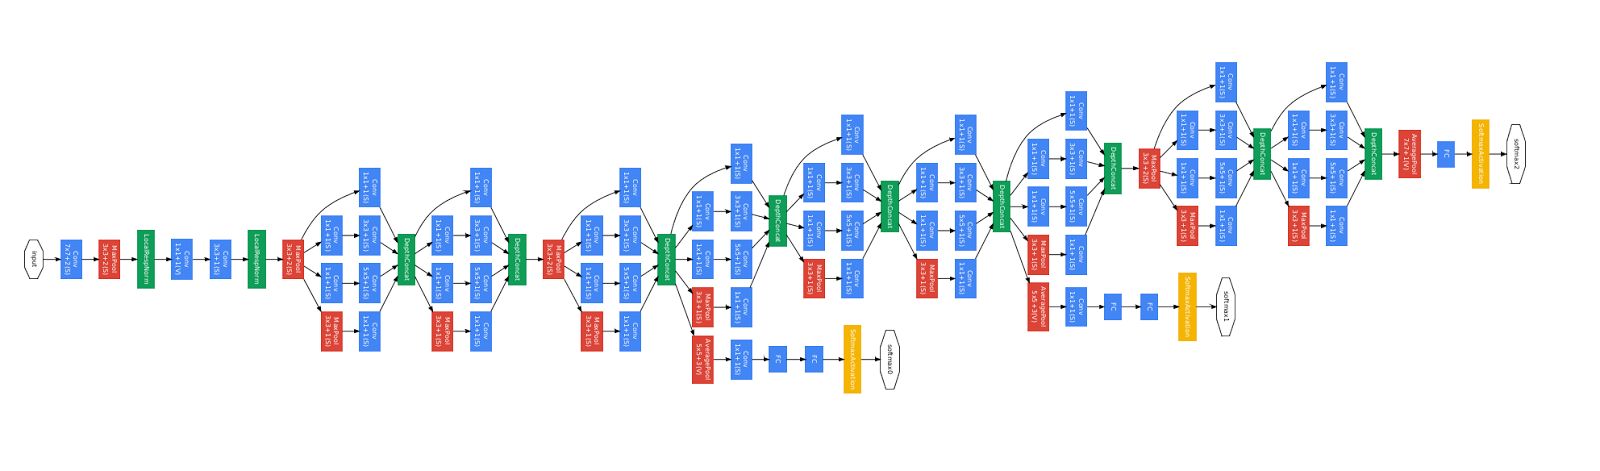
\includegraphics[width=0.7\linewidth]{image/GoogLeNet}
	\caption[]{GoogLeNet's architecture}
	\label{fig:googlenet}
\end{figure}

\subparagraph{Inception module}\mbox{}\\
Inception modules are used in GoogLeNet to allow for more efficient computation through a dimensionality reduction with stacked 1x1 convolutions. The modules were designed to solve the problem of computational expense, as well as overfitting, among other issues. The solution, in short, is to take multiple kernel filter sizes within the CNN, and rather than stacking them sequentially, ordering them to operate on the same level. 

As a neural net deals with a vast array of images, with wide variation in the featured image content, also known as the salient parts, they need to be designed appropriately. The most simplified version of an inception module works by performing a convolution on an input with not one, but three different sizes of filters (1x1, 3x3, 5x5). Also, max pooling is performed. Then, the resulting outputs are concatenated and sent to the next layer.
A method to reduce the number of computation is dimensionality reduction. This involves convolutions with 1x1 filters before convolutions with bigger filters.
\begin{figure}[h]
	\centering
	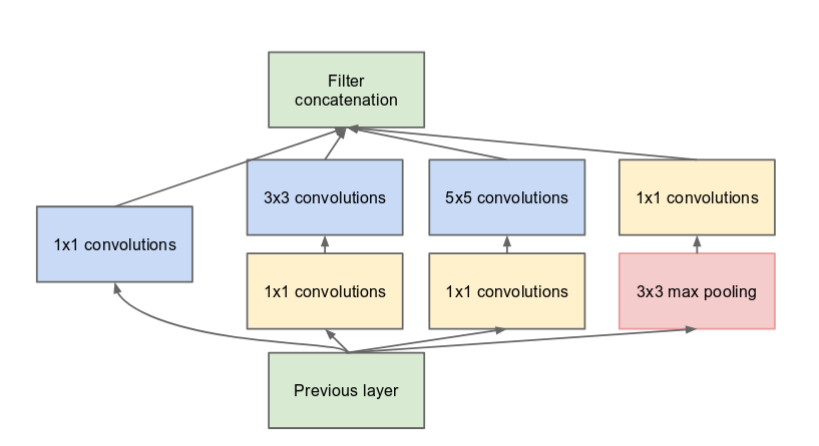
\includegraphics[width=0.7\linewidth]{image/inc_module}
	\caption{Inception module with dimension reduction}
	\label{fig:incmodule}
\end{figure}




\subparagraph{ResNeXt}
ResNeXt \cite{resnext} was the first runner up in ILSVRC 2016, achieving 3.03\% top-5 error rate, better than human precision on the same dataset (5,1\% error).The model name, ResNeXt, contains Next. It means the next dimension, on top of the ResNet, namely the winner in ILSVRC 2015. This next dimension is called the “cardinality” dimension.\\
The architecture adopts VGG/ResNets’ strategy of repeating layers, while
exploiting the split-transform-merge strategy (for example inception modules have the same approch, that is, input is split into a few lower-dimensional embeddings, transformed by a set of specialized filters, and merged by concatenation). 
A module in this network performs a set of transformations, each on a low-dimensional embedding, whose outputs are aggregated by summation. The transformations to be aggregated are all of the same topology (Figure \ref{fig:resnext_block} (right)).\\

\begin{figure}[h]
	\centering
	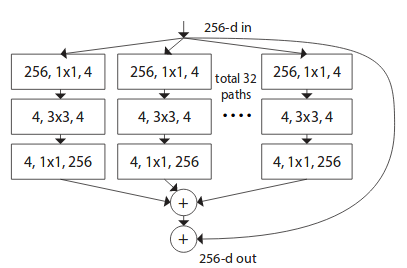
\includegraphics[width=0.7\linewidth]{image/resnext}
	\caption{Left: A block of ResNet. Right: A block of ResNeXt with cardinality=32. A layer is shown as (\# in channels, filter size, \# out channels)}
	\label{fig:resnext_block}
\end{figure}

Experiments in \cite{resneXt} demonstrate that increasing cardinality (the size of the set of transformations) is a more effective way of gaining accuracy than going deeper or wider, especially when depth and width starts to give diminishing returns for existing models.\\
In our work we use ResNeXt-50 32$\times$4d (Figure \ref{fig:res}), that represents a network with four bottleneck, and each layer having cardinality of 32. 

\begin{figure}
	\centering
	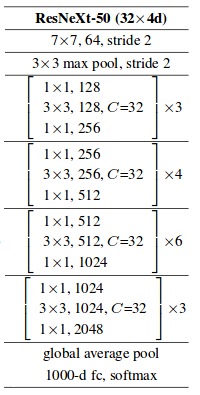
\includegraphics[height=0.4\linewidth]{image/res}
	\caption{ResNeXt-50 (32$\times$4)'s architecture}
	\label{fig:res}
\end{figure}
\section{Experiments}\label{experiments}

\subsection{Setup}
Both the built models and the experiments have been implemented in Pytorch (\cite{pytorch}). The reason why we chose this library is because of the presence of models, pretrained and not, that we wanted to study.\\
The training of the models and the experiments were performed on a virtual machine (VM) hosted by \textit{Compute Engine}, one of the services provided by Google Cloud Platform (\cite{gcloud}). Its configuration, shown in table \ref{table:specVM}, is a pre-setting provided by the service itself and designed for deep learning applications  (\cite{vmconfig}). The dataset was stored in a \textit{Google Cloud Storage}'s Bucket, another service provided by Google Cloud Platform.

\begin{table}
	\centering
	\begin{tabular}{|l|l|} 
		\hline
		\textbf{Component} & \textbf{Specification}  \\ 
		\hline
		OS                 & Debian 9                \\
		vCPU               & 2                       \\
		RAM                & 13GB                    \\
		GPU                & 1X NVIDIA Tesla K80     \\
		Disk               & 100GB                   \\
		Disk Type          & SSD                     \\
		Availability Zone  & us-west1-b              \\
		\hline
	\end{tabular}
\\
\caption{VM specifications}
   	\label{table:specVM}
\end{table}

\subsection{Implementation Details}\label{ImplDet}

For each CNN, we tested their performance with different learning rate values ($10^{-2}, 10^{-3}, 10^{-4}, 10^{-5}$). We have observed that $10^{-3}$ is the value which allows to converge faster to the best results, thus all experiments we have performed use this learning rate.\\
In figure \ref{fig:lr} we report ResNeXt's performance based on these different values, where it's clear that the lowest value of learning rate slows down the training phase, instead higher values ($10^{-2}$) bring more instability in the accuracy trend.

\begin{figure}[h]
	\centering
	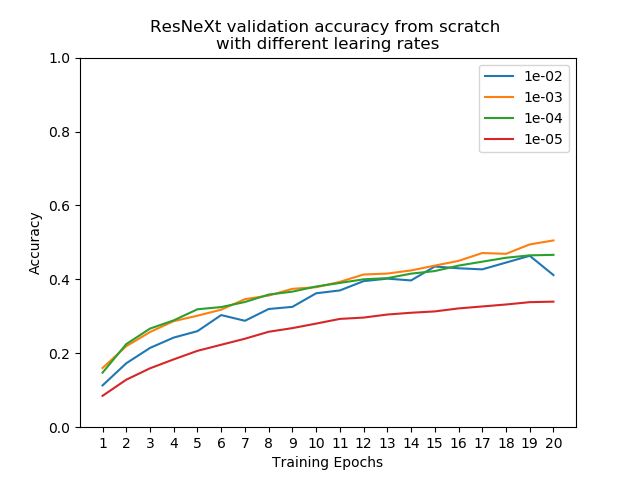
\includegraphics[width=.5\textwidth]{graphs/lr_scratch}\hfill
	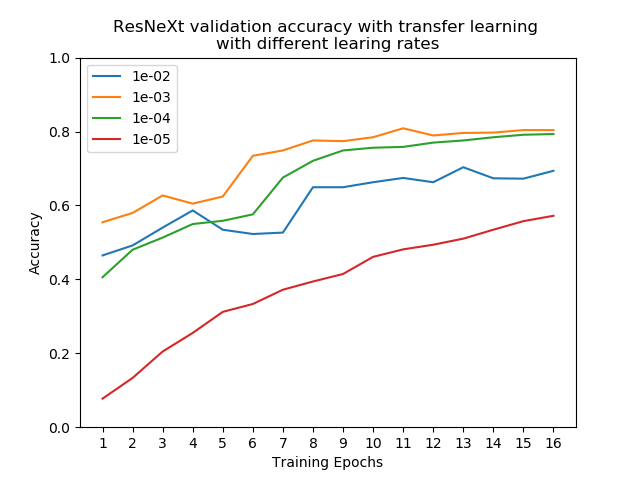
\includegraphics[width=.5\textwidth]{graphs/lr_tl}
	\caption{Top-1 accuracies for ResNeXt's validation set}
	\label{fig:lr}
\end{figure}

We chose the Adam's update rule because the experiments using SGD were worse. \textbf{Abbiamo impostato il }learning rate $= 10^{-3}$ mentre per gli altri papametri we used the default ones, i.e. $\beta_{1}  = 0.9$ and $\beta_{2} = 0.999$.  \textbf{MA COSA SONO beta1 e BETA2}\\

In transfer learning training, we set the number of epochs and the batch size to 16 and 32 respectively.  For each model chosen, pytorch makes available the final weights of these models trained on the ImageNet dataset (\cite{imagenet}), which makes transfer learning very easy to exploit.\\
We first start training the network updating the weights only in the FC-layers, but the results obtained weren't good.\\
With the aim of achieving higher accuracy, as experimented in \cite{ArtistIdCNN406}, we have decided to allow the update of the weights in the whole network if, for 3 consecutive epochs, the validation set's accuracy does not improve by 3 percentage points. When this condition occurs, learning rate is decreased by a factor of 10. This strong decrease is motivated by the fundamental idea in using transfer learning: it is assumed that the pre-trained weights are already "close" or enough good to those we are looking for, so it is good to search for them with a relatively small step-size.
\\

In training from scratch, the number of epochs was set to 21, while the batch size was still 32.\\ 
Weights' nitialisation follows a uniform distribution in $[-x, x]$ where $x=1/\sqrt n$ and $n$ is the number of inputs to a given neuron (\textbf{STA COSA È DA VERIFICARE})\\
We have experimented what in pytorch is called \textit{scheduler}, i.e. every 7 epochs the learning rate is decreased by a factor of 10 . This strategy, however, has not led to improvements and in fact the results exposed have been obtained without the use of this technique.

\subsection{Evaluation metrics}
In order to evaluate all the models that we study, we calculated their top-1 accuracy, which is when a paint is classified with its author, and top-3 accuracy, aka a paint is classified correctly when its author is one of the 3 artist to whom the model has assigned the highest scores.\\
Finally, we have compared our results with those in \textbf{CIT??}, which is/are the most related works with ours. 

The most significant results are reported in \ref{results}.

\subsection{Results}\label{results}

\textbf{RESNET SI SATURA PRIMA DI RESNEXT}

In table \ref{table} we report the overall results obtained for each CNN, both as regards training with transfer learning and the one from scratch, including in it the results obtained in \cite{ArtistIdCNN406} and \textbf{altri.}...

The first thing with we see, comparing the CNNs, is that AlexNet's performance are much worse than other CNNs for all experiments, thus we can deduce how network's complexity allows to achieve better results. In fact, GoogLeNet and ResNeXt are successors of AlexNet, so this results should not be surprising. 
In particular, in training from scratch, AlexNet is 20 percentage points worse than others CNNs, and in training with transfer learning this distance is halved. This result show that transfer learning performs very well in order to achieve discreet results even with not so complex networks. Indeed, AlexNet has obtained 87\% of top-3 accuracy in the test set.

For all the networks, we can see how training with transfer learning achieved results with 40 percentage points more than training from scratch. So, we can figure out that CNNs already trained on ImageNet dataset, which is wider than ours,  are a valuable starting point for artist identification and thus image classification and artist identification are tasks at least partially overlapped. \textbf{da riguardare}\\
The most performing CNN is ResNeXt trained with transfer learning. Its top-1 accuracy reaches 80\% on test set, while its top-3 accuracy is roughly 93\%. This mean that it can narrow down the artist to three in the vast majority of cases.

Figure \ref{fig:confusion} shows the confusion matrix concerning ResNeXt's classification. Each row represents the true artist and each column represents a predicted artist. Ideally, we want as many predictions as possible to be concentrated on the diagonal as this means that the network correctly predicted the true artist. The maximum possible value for a cell in the confusion matrix is 45, since there are 45 paintings per artist in the dataset.\\
In general, we can easily see how the majority of artifacts are well-classified thanks to the hottest colours on the diagonal cell, i.e. more than 30 paints are well classified to 45. \textbf{rivedere}

In particular, the artits better classified (44 to 45) are Eugene Bodin, Ivan Aivazovsky and Raphael Kirchner. In fact, even though these artists may belong to differents artistic movements and styles, they've always paints in a manner that depicts the world very close to reality (\textbf{figura ?? show some example}).\\
For example, Ivan Aivazovsky produced many portraits and landscapes, over half of all of his paintings are realistic depictions of coastal scenes and seascapes. \\
The manner of painting real scenario or objects makes artist classification very similar to image classification. Indeed, form our results we note that artists with this characteristic obtained an higher accuracy.

For the artists whose paints are often misclassified, we have noticed some common traits which follows.\\
Some of them belong to movements such as surrealism, cubism or expressionism, thus their artifacts are not depicting real scenario (\textbf{esempi}), making them harder to classify.
For example, Pablo Picasso, who founded the cubism movement, is the most misclassified artist (30 to 45).
  
The second reason leading to misclassification is the similarity  between different artists.\\
The most striking example regards Ilya Repin, in fact the model has classified Boris Kustodiev as authors of 8 Repin's artworks. That's not so surprising since Repin was the Kustodiev's teacher, influencing significantly his style. (\textbf{example}).

Another reason concerning artists whose produced paints with different style between them, as we can see in figure \textbf{REF} where Van Gogh's artworks are reported. This complicates furthermore the classification, leading to worse performance (accuracy on Van Gogh is 33 to 45).

In figure \ref{fig:accscratch}, for each CNN trained from scratch,  we report the top-1 accuracy trends on training and validation set. What we see is that both trends are very close each other, which proves a very low level of overfitting.
From this fact, we deduce that with a wider dataset and an higher number of epochs, we could be obtained better performances. For this reason, we have decided to test once our best network for 30 epochs. We didn't extend this kind of experiment to all networks due to our Google Cloud's limit resources. As we expected, ResNeXt's accuracy trend \textbf{kept increasing } without introducing overfitting, reaching 59\% top-1 and 81\% top-3 accuracy on test set.

In figure \ref{fig:acctransfer}, instead, we see the trends for each CNN trained with transfer learning. In all of them, after few epochs, an increase in the trend's slope is noted. This corresponds to the moment where to the network is able to update not only the FC-layers' weights, but also for them of the whole network as previous explained in \ref{ImplDet}. So we can deduce that pre-trained CNNs are trying to adapt to artist identification task.

Moreover, we can see that GoogLeNet and ResNeXt, aftew roughly 10 epochs, are affected by overfitting. In fact there's an incresing difference between test accuracy and validation accuracy, stating that fewer epochs could have been needed. \textbf{Comunque sia i risultati ottenuti sono migliori di quelli dei related works.}


% Please add the following required packages to your document preamble:

\begin{table}[]
	\begin{tabular}{|c|c|c|c|c|}
		\hline
		\multicolumn{5}{|c|}{\textbf{Training from scratch}}                                                          \\ \hline
		\multirow{2}{*}{\textbf{Network}} & \multicolumn{2}{c|}{\textbf{Top-1}} & \multicolumn{2}{c|}{\textbf{Top-3}} \\ \cline{2-5} 
		& Train acc        & Test acc         & Train acc        & Test acc         \\ \hline
		AlexNet                           & 0.23103          & 0.27439          & 0.46159          & 0.51304          \\ \hline
		GoogLeNet                         & 0.42669          & 0.46956          & 0.68285          & 0.70628          \\ \hline
		ResNeXt-50                        & \textbf{0.50531} & \textbf{0.50048} & \textbf{0.74275} & \textbf{0.74782} \\ \hline
		ResNet-18 \cite{ArtistIdCNN406}                    & 0.516            & 0.511            & 0.737            & 0,710            \\ \hline
	\end{tabular}
	\begin{tabular}{|c|c|c|c|c|}
		\hline
		\multicolumn{5}{|c|}{\textbf{Training with transfer learning}}                                                           \\ \hline
		\multirow{2}{*}{\textbf{Network}} & \multicolumn{2}{c|}{\textbf{Top-1}}  & \multicolumn{2}{c|}{\textbf{Top-3}} \\ \cline{2-5} 
		& Train acc        & Test acc          & Train acc         & Test acc        \\ \hline
		AlexNet                           & 0.7134           & 0.68695           & 0.88925           & 0.87439         \\ \hline
		GoogLeNet                         & 0.87536          & 0.80579           & 0.96787           & 0.92492         \\ \hline
		ResNeXt-50                        & \textbf{0.92125} & \textbf{0.82318} & \textbf{0.98695}  & \textbf{0.94879} \\ \hline
		ResNet-18 \cite{ArtistIdCNN406}                    & 0.907            & 0.777             & 0.973             & 0.898           \\ \hline
	\end{tabular}
	\label{table}
\end{table}


\begin{figure}[htp]
	
	\centering
	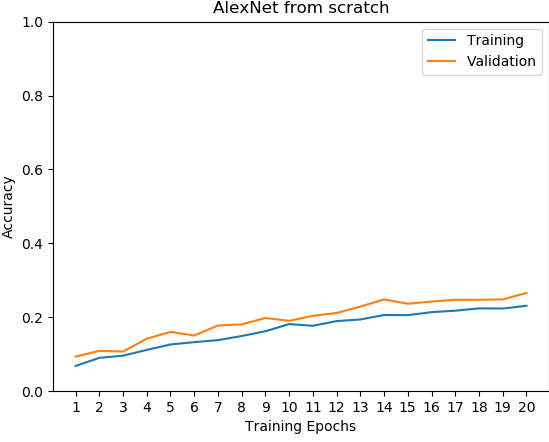
\includegraphics[width=.33\textwidth]{graphs/alex_scratch}\hfill
	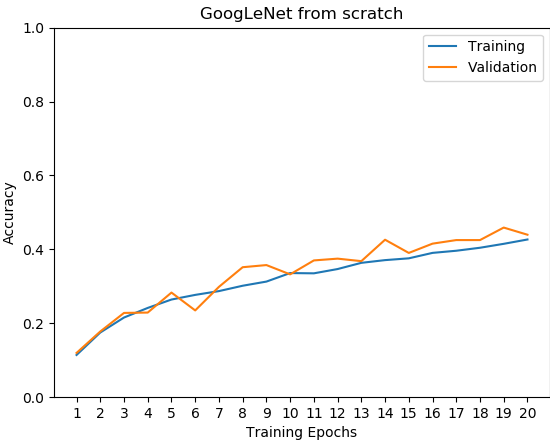
\includegraphics[width=.33\textwidth]{graphs/google_scratch}\hfill
	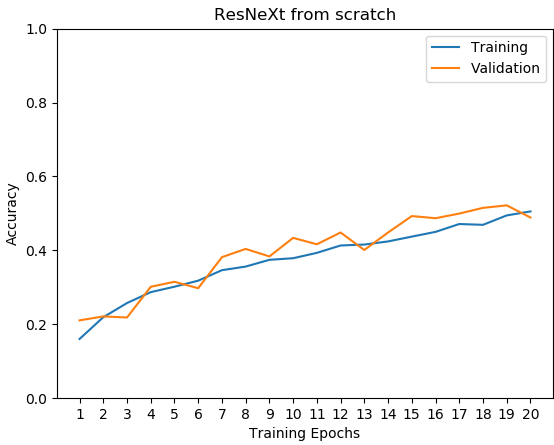
\includegraphics[width=.33\textwidth]{graphs/res_scratch}
	
	\caption{default}
	\label{fig:accscratch}
	
\end{figure}

\begin{figure}[htp]
	
	\centering
	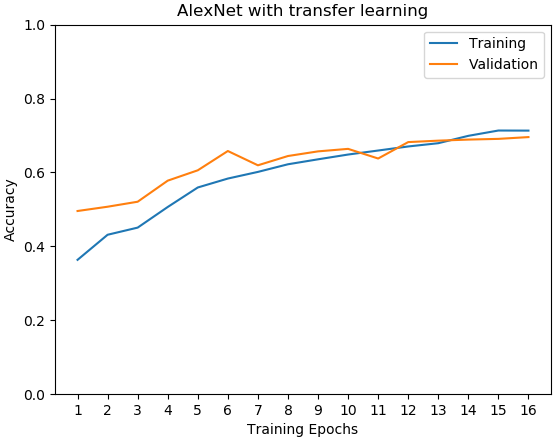
\includegraphics[width=.33\textwidth]{graphs/alex_training}\hfill
	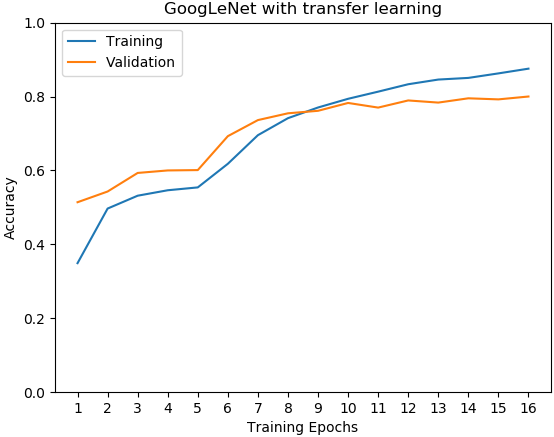
\includegraphics[width=.33\textwidth]{graphs/google_training}\hfill
	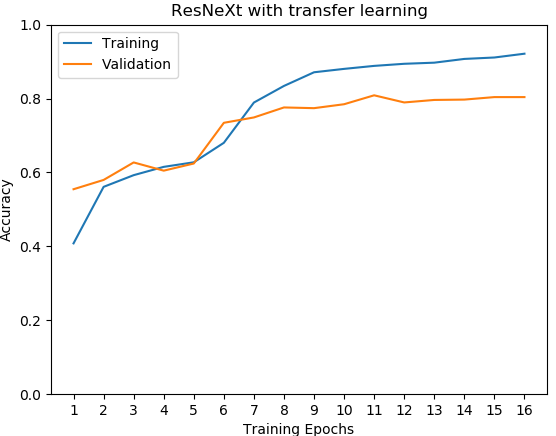
\includegraphics[width=.33\textwidth]{graphs/res_training}
	
	\caption{default}
	\label{fig:acctransfer}
	
\end{figure}

\begin{figure}
	\centering
	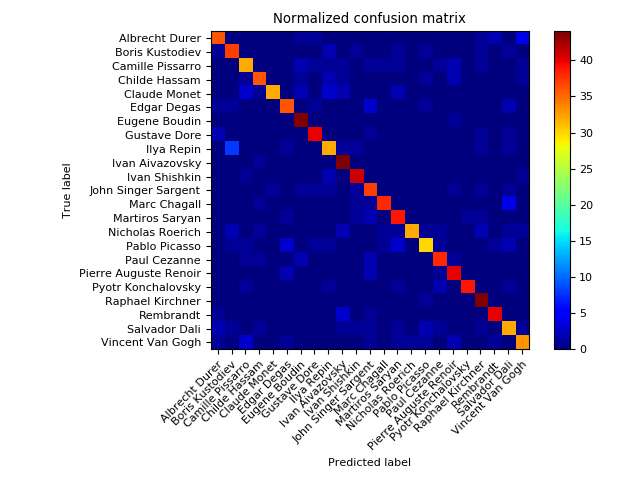
\includegraphics[width=0.8\linewidth]{graphs/confusion}
	\caption{Confusion matrix for top-1 classification on ResNeXt test set}
	\label{fig:confusion}
\end{figure}


\begin{figure}[htp]
	
	\centering
	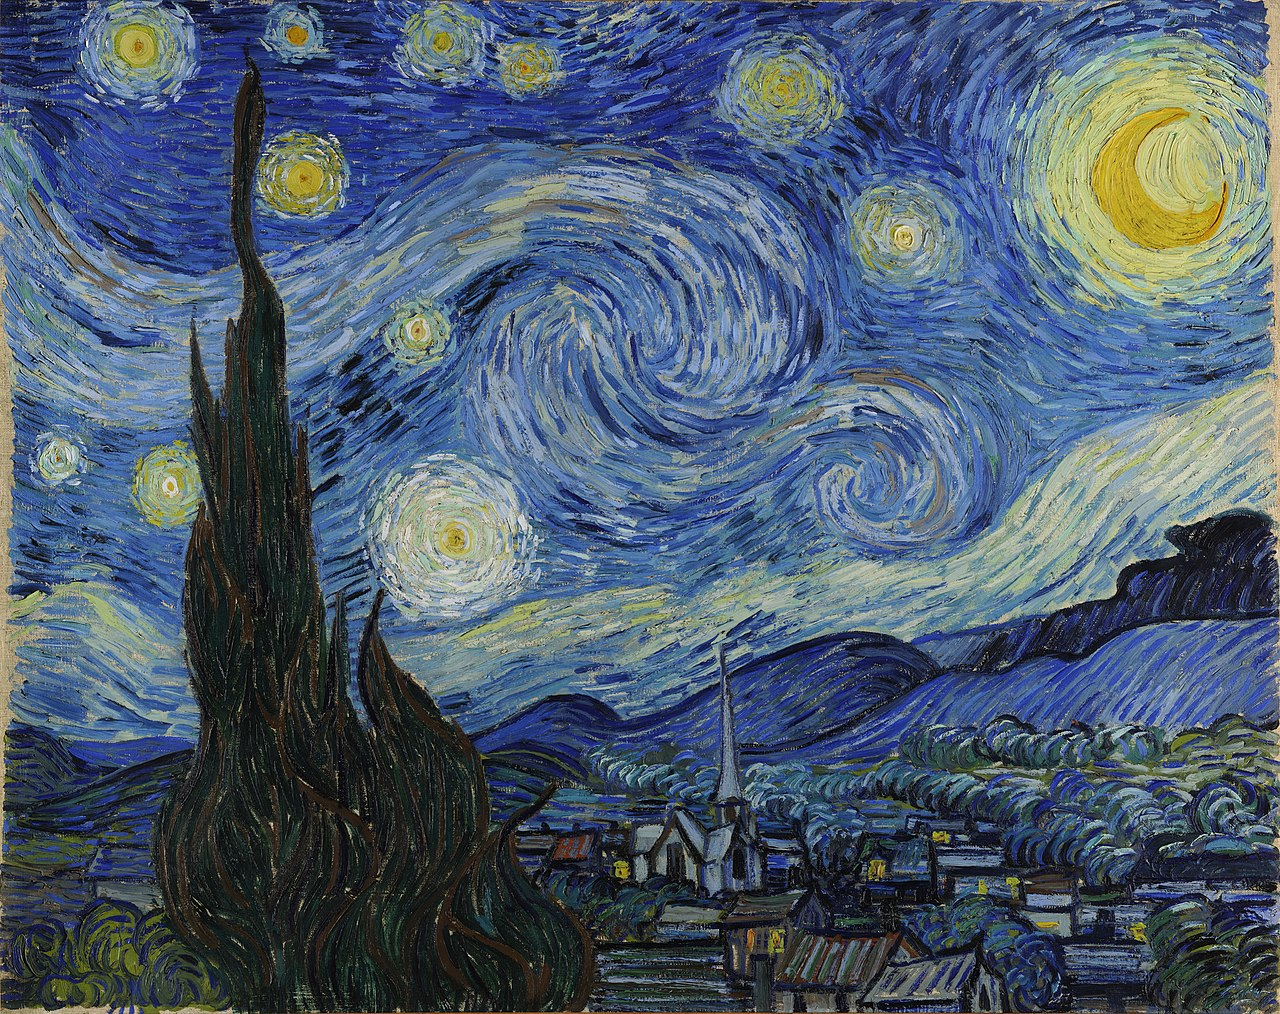
\includegraphics[width=.5\textwidth]{image/1280px-Van_Gogh_-_Starry_Night_-_Google_Art_Project}\hfill
	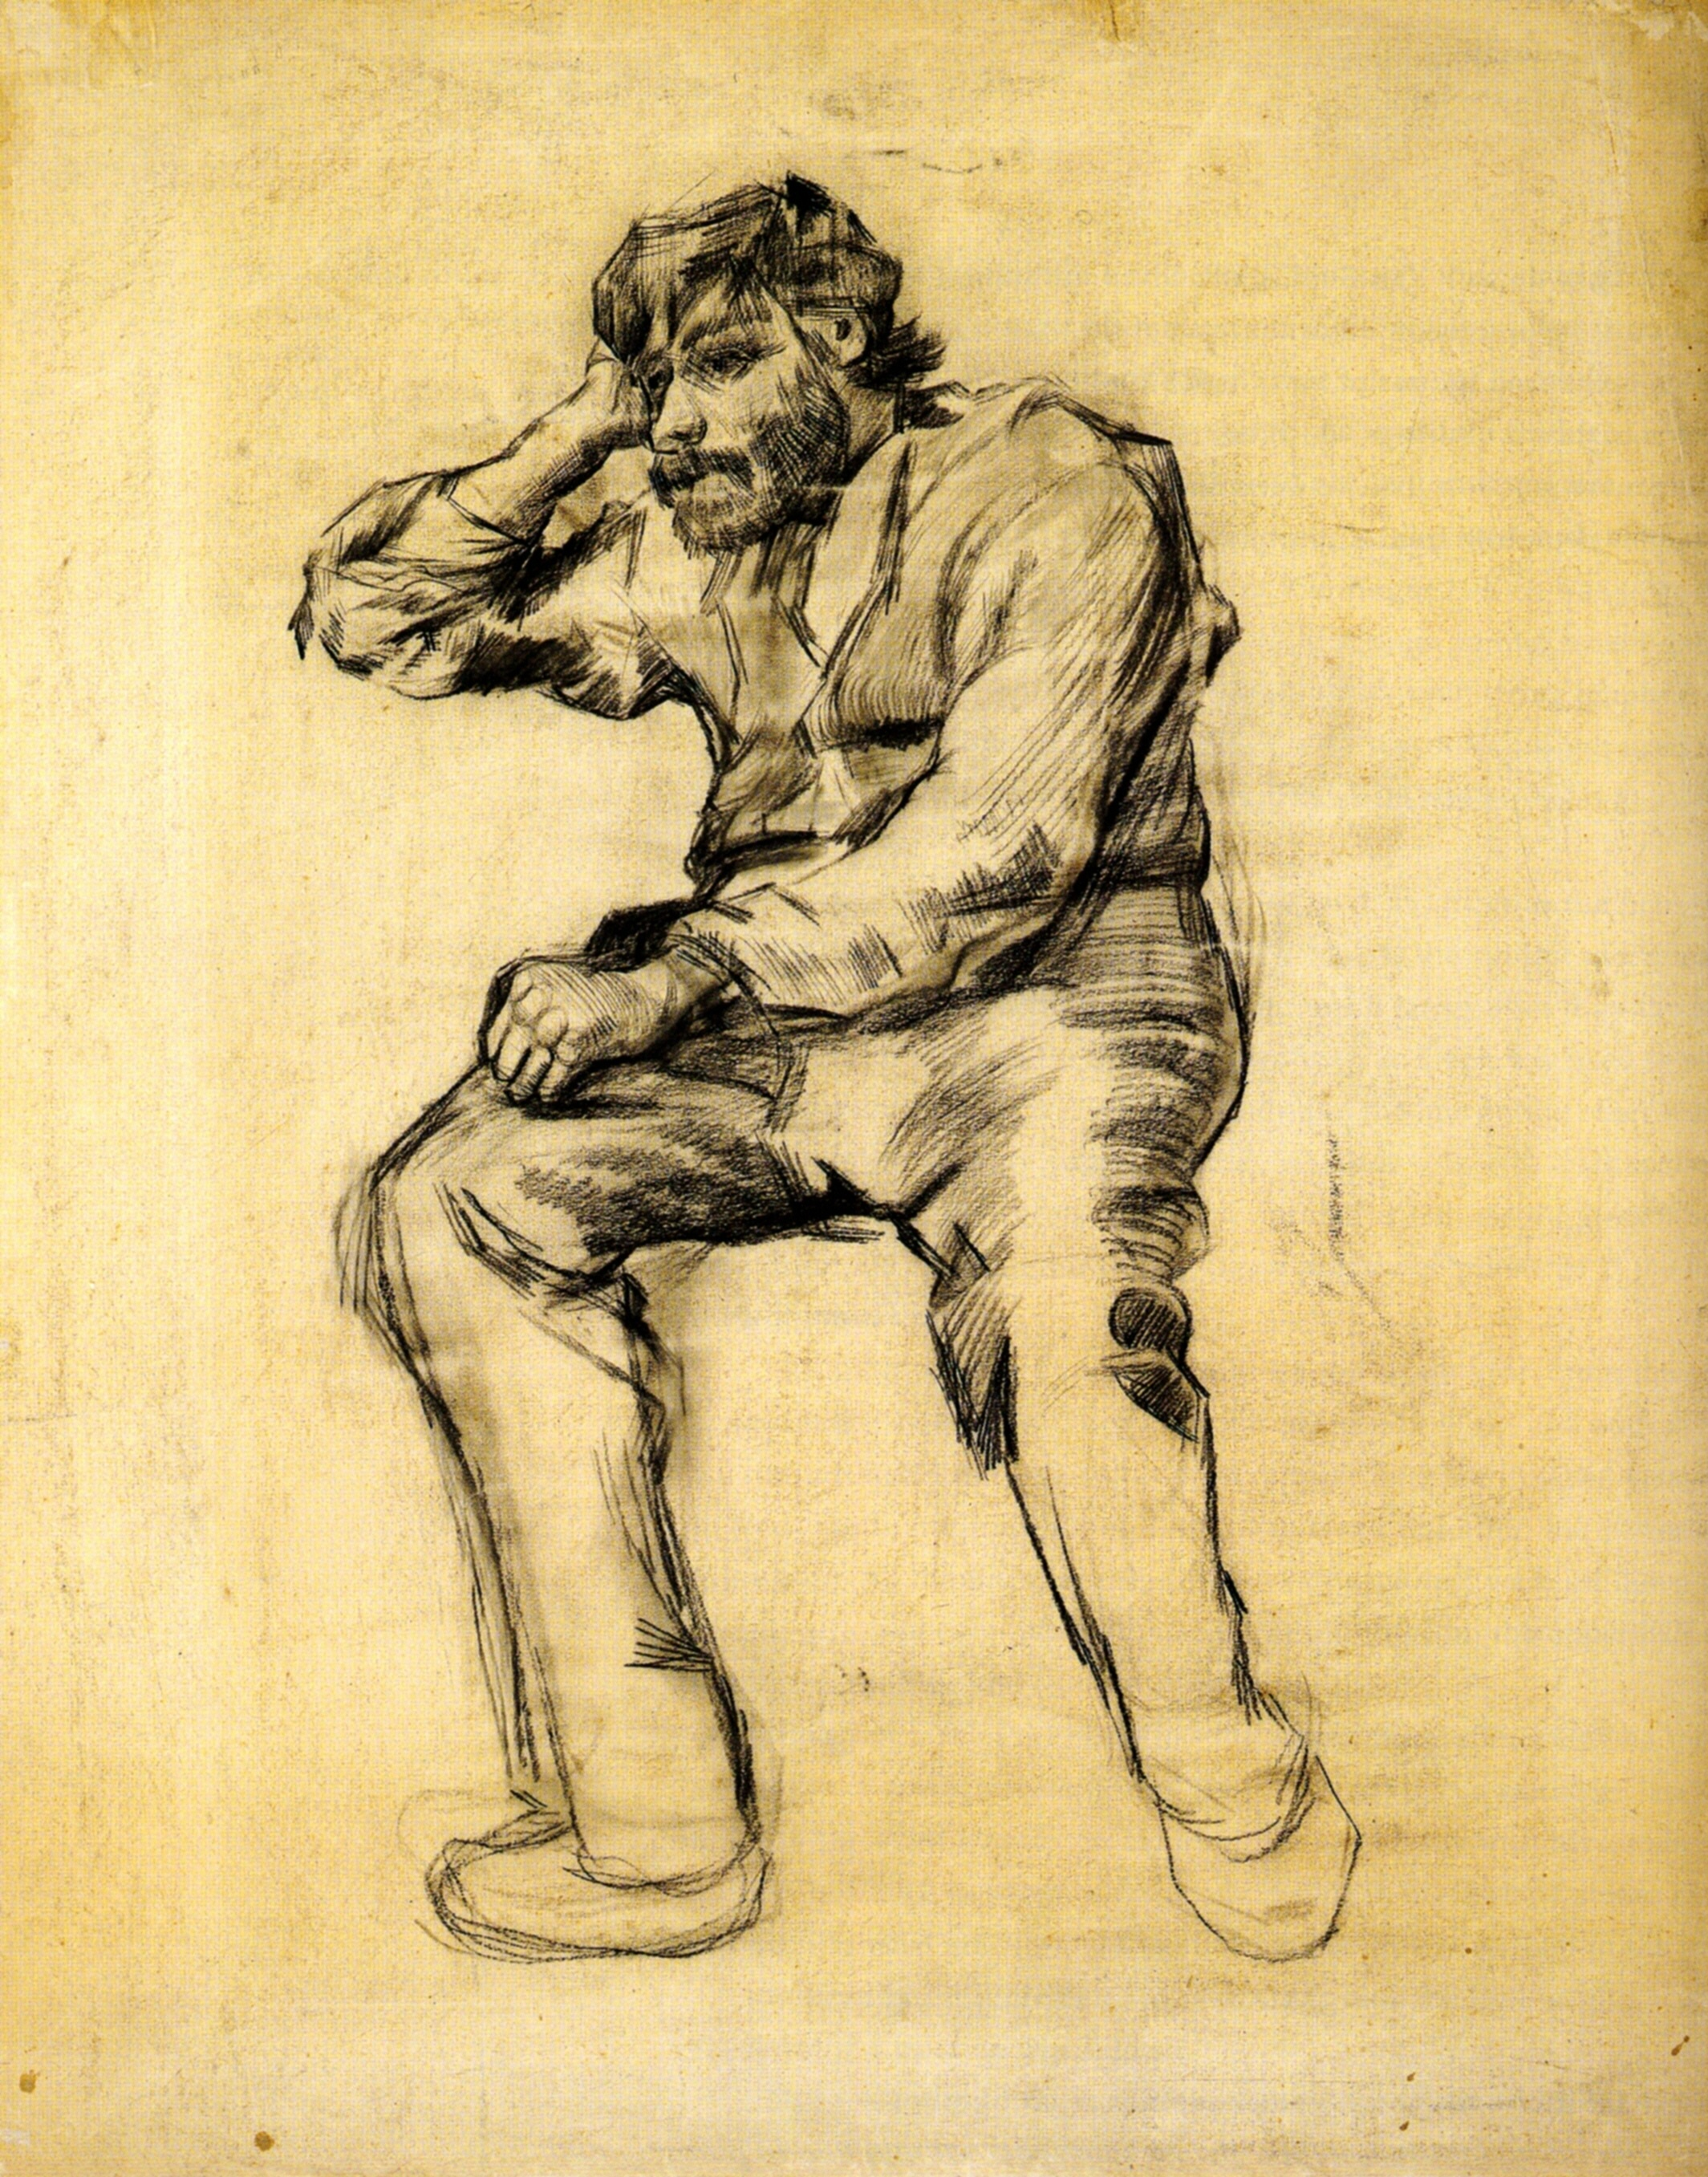
\includegraphics[height=.5\textwidth]{image/vincent-van-gogh_seated-man-with-a-beard-1886-1}
	
	\caption{default}
	\label{fig:vangogh}
	
\end{figure}

\section{Conclusions and future works}\label{conclusions}
In this essay we present the methods and approaches we have exploited to deal with artist identification. Once again we mark that it's a complex task, without lot of previous works. 
In our work we were able to reach a top-1 final accuracy of 82\% using ResNeXt with transfer learning, pre-trained on ImageNet, outperforming traditional feature-based approaches by a significant margin\textbf{ I REALTED WORK SU QUESTO TASK O SIMILI. FORSE DA AGGIUNGERE RESNEXT FROM SCRATCH.}. From these results we think that a larger dataset, both for number of paintings and artists, would allow a significantly increment in accuracy, particularly in training from scratch.

In future work we would like to deal with a task that could be considered related to this, namely the recognition of forgeries in art, starting from our work. Our belief is that the representation of style and content crated by our networks would be a good starting point to create a system able to assign a value of authenticity to a painting, because we think that, though is possible to replicate precisely an artifact, the style of an artist is somehow unique and possibly captured by a CNN.

%%% Comment out this section when you \bibliography{references} is enabled.
\begin{thebibliography}{1}
	
	\bibitem{hong2017}
	Yiyu Hong, Jongweon Kim, \newblock  Art Painting Identification using Convolutional Neural Network, \newblock International Journal of Applied Engineering Research, \newblock 2017
	
	\bibitem{Saleh2015}
	B. Saleh and A. M. Elgammal.\newblock  Large-scale classification
	of fine-art paintings: Learning the right metric on the right
	feature. \newblock CoRR, abs/1505.00855, 2015.
	\bibitem{Bar2014}
	W. L. Bar Y., Levy N. Classification of artistic styles using binarized features derived from a deep neural network.
	ECCV 2014.
	
	\bibitem{mensink2014}
	T. Mensink and J. van Gemert. \newblock The rijksmuseum challenge:
	Museum-centered visual recognition. \newblock 2014
	
	
	\bibitem{ArtistIdCNN406}
	Nitin Viswanathan, Standford University,
	\newblock Artist Identification with Convolutional Neural Networks, \newblock 2017
	
	\bibitem{ArtGANDataset}
	Dataset:
	\url{https://github.com/cs-chan/ArtGAN/tree/master/WikiArt Dataset}
	
	\bibitem{Lij2012}
	E. H. J. Li, L. Yao and J. Z. Wang. \newblock Rhythmic brushstrokes
	distinguish van gogh from his contemporaries: Findings via
	automated brushstroke extractions. IEEE Trans. Pattern
	Anal. Mach. Intell, \newblock 2012.
		
	\bibitem{lombardi05}
	T. E. Lombardi. \newblock The classification of style in fine-art painting. ETD Collection for Pace University, \newblock 2005.
	
	\bibitem{jou2011}
	J. Jou and S. Agrawal. Artist identification for renaissance
	paintings, 2011.
	\bibitem{razavian2014}
	A. H. S. J. C. S. Sharif Razavian, A. Cnn features off-theshelf: An astounding baseline for recognition, 2014.
	
	\bibitem{resnet}
	Kaiming He, Xiangyu Zhang, Shaoqing Ren, Jian Sun. Microsoft Research. 
	Deep Residual Learning for Image Recognition. 2015
	
	\bibitem{resneXt}
	Saining Xie, Ross Girshick, Piotr Dollar, Zhuowen Tu, Kaiming He. UC San Diego - Facebook AI Research. Aggregated Residual Transformations for Deep Neural Networks, 2017.
	
	\bibitem{googlenet}
	Christian Szegedy, Wei Liu, Yangqing Jia, Pierre Sermanet, Scott Reed, Dragomir Anguelov, Dumitru Erhan, Vincent Vanhoucke, Andrew Rabinovich. Going Deeper with Convolutions. 2014
	
	\bibitem{alexnet}
	Alex Krizhevsky, Ilya Sutskever, Geoffrey E. Hinton. ImageNet Classification with Deep Convolutional
	Neural Networks. 2012

	\bibitem{pytorchguide}
	Sasank Chilamkurthy.
	\url{https://pytorch.org/tutorials/beginner/transfer_learning_tutorial.html}
	
	\bibitem{dropout}
	G. E. Hinton, N. Srivastava, A. Krizhevsky, I. Sutskever and R. R. Salakhutdinov.
	Improving neural networks by preventing co-adaptation of feature detectors. 2012
	
	\bibitem{imagenet}
	ImageNet: \url{http://www.image-net.org/}
	
	\bibitem{pytorch}
	Pytorch: \url{https://pytorch.org/}
	
	\bibitem{vmconfig}
	Virtual Machine pre-settings: \url{https://console.cloud.google.com/marketplace/details/click-to-deploy-images/deeplearning}
	
	\bibitem{gcloud}
	Google Cloud Platform: \url{https://cloud.google.com/}

	
\end{thebibliography}


\end{document}